\documentclass[english]{article}
\usepackage[utf8]{inputenc}
\usepackage[T1]{fontenc}
\usepackage{babel}
\usepackage{amsmath}
\usepackage{graphicx}
\usepackage{fancyhdr}
\newcommand{\scidatalogo}{
\includegraphics[height=36pt]{SciData_logo.jpg}}
\newcommand{\overleaflogo}{
\includegraphics[height=36pt]{Overleaf-logo-300dpi.png}}
\pagestyle{fancy}
\fancyhf{}
\renewcommand{\headrulewidth}{0pt}
\setlength{\headheight}{40pt} 
\lhead{\textsc{\scidatalogo}}
\rhead{\textsc{\overleaflogo}}

\begin{document}

% Data Descriptor Title (110 character maximum, inc. spaces)
\title{Medical Information Mart for Intensive Care (MIMIC-III): the public access critical care database}

\author{
Firstname Lastname\textsuperscript{1}
, Firstname Lastname\textsuperscript{2{*}}
}

\maketitle
\thispagestyle{fancy}

1. An affiliation 2. A different affiliation {*}corresponding author(s):
Firstname Lastname (email@address)

\begin{abstract} % 170 words
MIMIC-III is a large, single-center database comprising information relating to patients admitted to critical care units at a large tertiary hospital. Data includes vital signs, medications, laboratory measurements, observations charted by clinicians, fluid balance, procedure codes, diagnostic codes, imaging reports, outcomes, and more. The highly detailed resource supports areas including academic and industry research, benchmarking of algorithms, and higher education coursework.
\end{abstract}

\section*{Background \& summary} % 700 words

% --- REQUIREMENTS OF THIS SECTION --- %
% (700 words maximum) An overview of the study design, the assay(s)
% performed, and the created data, including any background information
% needed to put this study in the context of previous work and the literature.
% The section should also briefly outline the broader goals that motivated
% the creation of this dataset and the potential reuse value. We also
% encourage authors to include a figure that provides a schematic overview
% of the study and assay(s) design. This section and the other main
% body sections of the manuscript should include citations to the literature
% as needed \cite{cite1, cite2}. References should be included within the 
% manuscript file itself as our system cannot accept BibTeX bibliography files. 
% Authors who wish to use BibTeX to prepare their references should therefore 
% copy the reference list from the .bbl file that BibTeX generates and paste it 
% into the main manuscript .tex file (and delete the associated 
% \textbackslash{}bibliography and \textbackslash{}bibliographystyle commands).
% ------------------------------------ %

In recent years there has been a concerted move towards the adoption of digital health record systems in hospitals. In the US, for example, the number of non-federal acute care hospitals with basic digital systems increased from 9.4\% to 75.5\% over the 7 year period between 2008 and 2014 \cite{cite1}.

Despite this advance, interoperability of digital systems and archiving of data remain inadequate. As a result, the potential that hospital data offers in terms of understanding and improving care is yet to be fully realised. In parallel, the scientific research community is increasingly coming under criticism for the lack of reproducibility of studies \cite{cite2}.

Here we report release of the MIMIC-III database, an update to the widely-used MIMIC-II database \cite{cite3}. MIMIC-III integrates inaccessible clinical data and makes it widely accessible to researchers internationally (Figure \ref{fig:mimicoverview}). By allowing data and code used for its analysis to be shared together, the database allows studies to be reproduced and critiqued in ways that would not otherwise be possible. 

Based on our experience of the previous major release of MIMIC (MIMIC-II, released in 2010) we anticipate MIMIC-III to be widely used internationally in areas such as academic and industry research, benchmarking of algorithms, and higher education coursework.

The MIMIC-III critical care database is unique and notable for the following reasons: 
\begin{itemize}
  \item it is the only freely accessible database of its kind;
  \item the dataset is large and highly granular, with detailed information about individual patient care;
  \item access is unrestricted by institutional barriers, enabling clinical research and education around the world.
\end{itemize}

\subsection*{Patient characteristics}

MIMIC-III comprises data associated with patients admitted to critical care units of the Beth Israel Deaconess Medical Center in Boston, Massachusetts, between 2001 and 2012. The data...describe the details after generating table (Table \ref{table:patientpopulation}).

The five most common International Classification of Disease codes across all critical care units were: X, X, X, X, and X. Table \ref{table:icddistribution} gives an indication of how different diseases, as indicated by the primary ICD-9 code, are distributed across the critical care units. 

NB: There are 13 distinct care units in MIMIC-III, so we will need to decide how to incorporate these into Tables 1 and 2: CSICU; SICU; NSICU; NICU; MICU; MSICU; CCU; CTICU; TSICU; NWARD; CVICU; SICU Nursing. \\

FIGURE: Demonstrate the structure of the patient population. \\

FIGURE: ICD9 codes \\

% \subsection*{Roadmap}

% To maximise research potential, the database will be iteratively enhanced over subsequent minor releases. For example, we anticipate later versions of the database to incorporate data from the emergency care department of Beth Israel Deaconess Medical Center.

% In the more distant future we seek to create a federated database by linking MIMIC-III with international hospital databases. Progress has been made towards this aim in collaboration with several hospitals in Europe and South America.

\subsection*{Classes of data}

Data available in the MIMIC-III database ranges from time-stamped, nurse-verified physiological measurements made at the bedside to free-text interpretations of imaging studies provided by the radiography department. Table \ref{table:dataclasses} gives an overview of the different classes of data available. 

\section*{Methods}

% --- REQUIREMENTS OF THIS SECTION --- %
% The Methods should include detailed text describing any steps or procedures 
% used in producing the data, including full descriptions of the experimental 
% design, data acquisition assays, and any computational processing (e.g. 
% normalization, image feature extraction). Related methods should be grouped 
% under corresponding subheadings where possible, and methods should be described 
% in enough detail to allow other researchers to interpret and repeat, if required, 
% the full study. Specific data outputs should be explicitly referenced via data 
% citation (see Data Records and Data Citations, below). Authors should 

% previous descriptions of the methods under use, but ideally the method 
% descriptions should be complete enough for others to understand and reproduce 
% the methods and processing steps without referring to associated publications. 
% There is no limit to the length of the Methods section.
% ------------------------------------ %

The Laboratory for Computational Physiology at Massachusetts Institute of Technology is an interdisciplinary team of data scientists and practicing physicians, allowing clinical input to guide technical development. MIMIC-III is the third iteration of the MIMIC critical care database, enabling us to draw upon prior experience \cite{cite3}. 

\subsection*{Database development}

The database was populated with data from existing archiving systems that had been acquired during routine hospital care, so there was no associated burden on carers and no interference with treatment of patients. 

The project was approved by the Institutional Review Boards of Beth Israel Deaconess Medical Center (Boston, MA) and the Massachusetts Institute of Technology (Cambridge, MA). Requirement for individual patient consent was waived because the study did not impact clinical care and all protected health information was deidentified.

Two different critical care information systems were in place over the data collection period: Philips CareVue Clinical Information System (models M2331A and M1215A; Philips Health-care, Andover, MA) and iMDsoft MetaVision ICU (iMDsoft, Needham, MA). These systems were the source of clinical data such as: 
\begin{itemize}
  \item time-stamped nurse-verified physiological measurements (for example, hourly documentation of heart rate, arterial blood pressure, respiratory rate, etc).
  \item caregiver documented progress notes.
  \item continuous intravenous drip medications and fluid balances.
\end{itemize}

Additional information was collected from the hospital health record system, including, such as:
\begin{itemize}
  \item laboratory test results (for example, complete blood counts, and microbiology results).
  \item patient demographics and in-hospital mortality.
  \item billing-related information such as International Classification of Disease, 9th Edition (ICD-9) codes, Diagnosis Related Group (DRG) codes, and Current Procedural Terminology (CPT) codes.
\end{itemize}
Out-of-hospital mortality dates were obtained using the Social Security Administration Death Master Files. A more detailed description of the data is shown in Table 1. 

\subsection*{Deidentification}

Before data was incorporated into the MIMIC-III database, it was first deidentified according to Health Insurance Portability and Accountability Act (HIPAA) standards using structured data cleansing and date shifting. The deidentification process for structured data required the removal of all eighteen of the identifying data elements, including fields such as patient name, telephone number, and address. We also removed provider identifiers.

Protected health information was removed from free text fields such as diagnostic reports and physician notes using an updated version of an algorithm that has been shown to have superior performance in comparison to clinicians in detecting protected health information \cite{cite5}.

\subsection*{Data access}

MIMIC-III contains detailed information regarding the clinical care of patients, so it must be treated with appropriate care and respect. Researchers are required to formally request access via a process documented on MIMIC website. There are two key steps that must be completed before access is granted:

\begin{enumerate}
  \item the researcher must complete a recognised course in protecting human research participants.
  \item the researcher must sign a Data Use Agreement, which outlines appropriate data usage, security, and forbids efforts to identify individual patients.
\end{enumerate}

Approval requires at least a week. Once an application has been approved the researcher will receive emails containing instructions for downloading the database from PhysioNetWorks \cite{cite6}. 

\subsection*{Code availability}

% --- REQUIREMENTS OF THIS SECTION --- %
%For all studies using custom code in the generation or processing of datasets, 
%a statement must be included here, indicating whether and how the code can be 
%accessed, including any restrictions to access. This section should also include 
%information on the versions of any software used, if relevant, and any specific 
%variables or parameters used to generate, test, or process the current dataset. 
% ------------------------------------ %

The code used to create the MIMIC-III database from raw hospital exports has been made available in a public archive. Prior to opening up the code, the commit history was deleted to avoid sensitive information being inadvertently shared: https://github.com/MIT-LCP/mimic-iii-building 

The code that underpins the MIMIC-III website and documentation is also openly available and contributions from the research community are encouraged: \\ https://github.com/MIT-LCP/mimic-website 

Additionally, a public "MIMIC Code Repository" has been created to encourage researchers to collaboratively develop and share code used for data processing and analysis: https://github.com/MIT-LCP/mimic-code

% Answer:
% Deidentification code available at github.com/MIT-lcp/deid

\section*{Data records}

% --- REQUIREMENTS OF THIS SECTION --- %
% Please explain each data record associated with this work, including
% the repository where this information is stored, and an overview of
% the data files and their formats. Each external data record should
% be listed in Data Citation section at the end of this template, and 
% records should be cited throughout the manuscript as, for example 
% (Data Citation 1). 

% Tables should be used to support the data records, and should clearly indicate 
% the samples and subjects, their provenance, and the experimental manipulations 
% performed on each. They should also specify the data output resulting from each 
% data-collection or analytical step, should these form part of the archived record. 
% Please see the submission guidelines at the \emph{Scientific Data} website, and 
% our Word templates for more information on preparing such tables. 
% ------------------------------------ %

% Probably the most reasonable format:
% CHARTEVENTS, IOEVENTS, DATETIMEEVENTS from two ICU databases
% LABEVENTS from patient's medical record, spans across all their (?in-network) visits
% ADMISSIONS from hospital level admission/discharge/transfer information
% ICUSTAYEVENTS derived from ADMISSIONS
% DIAGNOSES_ICD from hospital billing database
% PROCEDURES_ICD from hospital billing database
% DRGCODES from hospital billing database
% NOTEEVENTS from hospital note entry database
% POE_MED_ORDER from provider order entry database (hospital wide)
% CALLOUT from hospital discharge planning database
% CAREGIVERS merged from the two ICU databases
% CPTEVENTS from hospital billing database
% D_ICD_DIAGNOSES, D_ICD_PROCEDURES, D_CPT from openly available sources
% D_LABITEMS from the same data that the labs were derived - the ITEMIDs were generated by us
% PATIENTS is derived from ADMISSIONS
% MICROBIOLOGYEVENTS ??
% SERVICES from hospital database
% TRANSFERS is the hospital ADT data

% Include a nice visualization of the data

MIMIC-III is a relational database consisting of 25 tables. Tables are linked by identifiers which usually have the suffix "ID". For example, SUBJECT\_ID refers to a unique patient, HADM\_ID refers to a unique admission to the hospital, and ICUSTAY\_ID refers to a unique admission to an intensive care unit. 

Charted events such as notes, laboratory tests, and fluid balance are stored in a series of "events" tables. For example the OUTPUTEVENTS table contains all measurements related to output for a given patient, while the LABEVENTS table contains laboratory tests for a patient.

Tables prefixed with “D\_” are dictionaries and provide definitions for identifiers. For example, every row of OUTPUTEVENTS is associated with a single ITEMID which represents the concept measured, but it does not contain the actual name of the drug. By joining OUTPUTEVENTS and D\_ITEMS on ITEMID, it is possible to identify what concept a given ITEMID represents. Further detail is provided below.

\subsection*{Data tables}

The following tables are used to define and track patient stays:

\begin{itemize}
  \item PATIENTS: Every unique patient in the database (defines SUBJECT\_ID).
  \item ADMISSIONS: Every unique hospitalization for each patient in the database (defines HADM\_ID).
  \item ICUSTAYS: Every unique ICU stay in the database (defines ICUSTAY\_ID).
  \item SERVICES: The clinical service under which a patient is registered.
  \item TRANSFERS: Patient movement from bed to bed within the hospital, including ICU admission and discharge.
\end{itemize}

The following tables contain data associated with each patient:

\begin{itemize}
  \item CALLOUT: Information regarding when a patient was cleared for ICU discharge and when the patient was actually discharged.
  \item CAREGIVERS: Every caregiver who has recorded data in the database (defines CGID).
  \item CHARTEVENTS: All charted observations for all patients.
  \item CPTEVENTS: Procedure codes for all procedures done for patients in the ICU.
  \item DATETIMEEVENTS: All recorded observations which are dates, for example time of dialysis or insertion of lines. These observations have been anonymized.
  \item DIAGNOSES\_ICD: Hospital assigned diagnoses as classified by the international classification of diseases and related health problems (ICD).
  \item DRGCODES: Diagnosis Related Groups (DRG) which are used for hospital billing for patient stays.
  \item INPUTEVENTS\_CV: Intake for patients monitored using the Philips CareVue system.
  \item INPUTEVENTS\_MV: Intake for patients monitored using the iMDSoft MetaVision system.
  \item OUTPUTEVENTS: Output information for patients while in the ICU.
  \item LABEVENTS: Laboratory measurements for patients both within the hospital and in outpatient clinics following hospital discharge.
  \item MICROBIOLOGYEVENTS: Microbiology measurements and antibiotic sensitivities from the hospital database.
  \item NOTEEVENTS: De-identified notes, including nursing and physician notes, ECG reports, imaging reports, and discharge summaries.
  \item PRESCRIPTIONS: Medications ordered for a given patient.
  \item PROCEDURES\_ICD: Patient procedures performed as coded by the international classification of diseases and related health problems (ICD) system.
\end{itemize}

The following tables are dictionaries:

\begin{itemize}
  \item D\_CPT: High level dictionary of Current Procedural Terminology (CPT) codes.
  \item D\_ICD\_DIAGNOSES: Brief description for each ICD code related to a diagnosis.
  \item D\_ICD\_PROCEDURES: Brief description for each ICD code related to a procedure.
  \item D\_ITEMS: Describes each ITEMID in the ICU database.
  \item D\_LABITEMS: Describes each ITEMID in the laboratory database.
\end{itemize}


\section*{Technical validation}

% --- REQUIREMENTS OF THIS SECTION --- %
% This section presents any experiments or analyses that are needed
% to support the technical quality of the dataset. This section may
% be supported by up figures and tables, as needed. This is a required
% section; authors must present information justifying the reliability
% of their data.
% ------------------------------------ %

A minimal amount of processing was undertaken to achieve the desired deidentification and data structure, helping to ensure that MIMIC-III closely represents the raw data collected within the Beth Israel Deaconess Medical Center.

Values derived from the raw hospital data, such as computed severity of illness scores, are not included in the core MIMIC-III data. Instead this supplementary information will be developed collaboratively by the community and labeled explicitly.

Best practice for scientific computing was followed where possible \cite{cite4}. Code used to build MIMIC-III was version controlled and developed collaboratively within the laboratory. The approach encouraged readable code and documentation, as well as frequent feedback from colleagues.

Issue tracking is used to ensure that limitations of the dataset and code are clearly documented and are dealt with as appropriate. The research community is encouraged to report and address issues as they are found, and a system for releasing minor database updates is in place.

% TP: some measures of quality might include: 
% TBC...
% Prior to release internal testing. Descriptive analysis conducted to ensure known features 
% of the patient population were represented by the data.
% 	Data imported successfully to PostgreSQL
% 	All ICUSTAY_ID associated with HADM_ID, all HADM_ID associated with a SUBJECT_ID
% 	No ages < 0
%	Very few DODs < discharge

\section*{Usage notes}

% --- REQUIREMENTS OF THIS SECTION --- %
% Brief instructions that may help other researchers reuse these dataset.
% This is an optional section, but strongly encouraged when helpful
% to readers. This may include discussion of software packages that
% are suitable for analyzing the assay data files, suggested downstream
% processing steps (e.g. normalization, etc.), or tips for integrating
% or comparing this with other datasets. If needed, authors are encouraged
% to provide code, programs, or data processing workflows when they may help 
% others analyse the data. We encourage authors to archive related code in 
% a DOI-issuing archive when possible, but code may also be supplied as 
% supplementary information files. 

% For studies involving privacy or safety controls on public access
% to the data, this section should describe in detail these controls,
% including how authors can apply to access the data, and what criteria
% will be used to determine who may access the data, and any limitations
% on data use. 
% ------------------------------------ %

MIMIC is provided as a collection of comma separated value (CSV) files, along with scripts to help with importing the data into popular database systems including PostreSQL and MySQL. Our laboratory is also trialing a shared cloud instance of the database which is made accessible to researchers on request. 

\subsection*{Community support}

Sharing a dataset such as MIMIC-III carries both a responsibility to address issues with the data, and an expectation from users to provide support. Our laboratory is committed to continuously improving the data and documentation, but resources limit the amount of tailored advice that we can give to the worldwide community of users.

We believe that some of the burden of support must be carried by the community as a whole. We have therefore made the repository used to generate the documentation and website publicly available and we encourage participation in its development. A forum for users to ask and answer MIMIC-III related questions is also due to be released.

% Our hope is that we can provide access while not covering compute costs...

\subsection*{Collaborative research}

Our experience is that many researchers work independently to produce code for data processing and analysis. We seek to move towards a more collaborative, iterative development process where researchers work together on a shared code base. To facilitate collaboration, we have created the MIMIC Code Repository.

The repository provides a place for researchers to share and reuse MIMIC related code. Examples of code already shared include a script to identify a sepsis cohort with the Angus criteria and a script to measure comorbidities using the Elixhauser Comorbidity Index. Over time, we expect the repository to become increasingly important for researchers working with MIMIC-III.

% TP: we may want to assign a DOI to the MIMIC Code Repository. This would allow it to be moved in future and also allow us to track citations etc.

\section*{Acknowledgements}

% --- REQUIREMENTS OF THIS SECTION --- %
% Text acknowledging non-author contributors. Acknowledgements should
% be brief, and should not include thanks to anonymous referees and
% editors, or effusive comments. Grant or contribution numbers may be
% acknowledged. Author contributions Please describe briefly the contributions
% of each author to this work on a separate line. 
% ------------------------------------ %

This research and development was supported by Critical Care Informatics Grants NIH-R01-EB017205, NIH-R01-EB001659, and NIH-R01-GW104987 from the National Institutes of Health. The authors would also like to thank Philips Healthcare and staff at the Beth Israel Deaconess Medical Center, Boston.

\section*{Competing financial interests}

The authors declare no competing financial interests.

\section*{Figures legends}

% --- REQUIREMENTS OF THIS SECTION --- %
% Figure should be referred to using a consistent numbering scheme through
% the entire Data Descriptor. For initial submissions, authors may choose
% to supply this document as a single PDF with embedded figures, but
% separate figure image files must be provided for revisions and accepted
% manuscripts. In most cases, a Data Descriptor should not contain more
% than three figures, but more may be allowed when needed. We discourage
% the inclusion of figures in the Supplementary Information \textendash{}
% all key figures should be included here in the main Figure section. 

% Figure legends begin with a brief title sentence for the whole figure
% and continue with a short description of what is shown in each panel,
% as well as explaining any symbols used. Legend must total no more
% than 350 words, and may contain literature references. 
% ------------------------------------ %

\begin{center}
\begin{figure}
\caption{Overview of the MIMIC-III critical care database.}
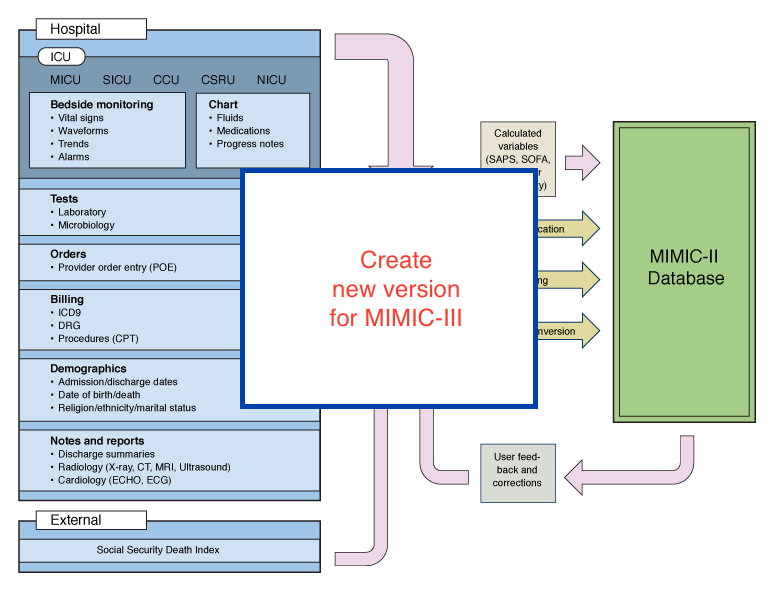
\includegraphics[width=\textwidth]{mimic.png}
\label{fig:mimicoverview}
\end{figure}
\end{center}

\section*{Tables}

% Tables supporting the Data Descriptor. These can provide summary information
% (sample numbers, demographics, etc.), but they should generally not
% be used to present primary data (i.e. measurements). Tables containing
% primary data should be submitted to an appropriate data repository. 

% Tables may be provided within the \LaTeX{} document or as separate
% files (tab-delimited text or Excel files). Legends, where needed,
% should be included here. Generally, a Data Descriptor should have
% fewer than ten Tables, but more may be allowed when needed. Tables
% may be of any size, but only Tables which fit onto a single printed
% page will be included in the PDF version of the article (up to a maximum
% of three). 

% Maximum of three tables included in the PDF (up to 10 in total)

% Table 1:
%	Overview of MIMIC-III

\begin{center}
\begin{table}
\begin{tabular}{|l|p{8cm}|}
    \hline
    Class of data & Description \\ 
    \hline
    Descriptive & Demographic detail, admission and discharge times, and dates of death. \\ 
    \hline
    Procedure and billing & Current Procedural Terminology (CPT) codes, Diagnosis-Related Group (DRG) codes, and International Classification of Diseases (ICD) codes. \\ 
    \hline
    Physiological & Nurse-verified vital signs, approximately hourly (e.g. heart rate, blood pressure, respiratory rate). \\ 
    \hline
    Laboratory & Blood chemistry, urine analysis, and microbiology test results. \\ 
    \hline
    Medications & Administration records of intravenous medications and ordered medications. \\ 
    \hline
    Imaging reports & Free text reports of imaging studies, such as echocardiograms and x-rays. \\ 
    \hline
    Notes & Free text notes such as carer progress notes and hospital discharge summaries. \\ 
    \hline
\end{tabular}
\caption{Classes of data available in the MIMIC-III critical care database.}
\label{table:dataclasses}
\end{table}
\end{center}

% Table 2:
%	Demographics of the database
\begin{center}
\begin{table}
\begin{tabular}{|p{5cm}|c|c|c|c|c|}
    \hline
    Critical care unit & MICU & SICU & CSRU & CCU & Total \\ 
    \hline
    Hospital admissions, no. (\% of total admissions) & N(N\%) & N(N\%) & N(N\%) & N(N\%) & N(N\%) \\ 
    \hline
    Distinct ICU stays, no. (\% of total admissions) & N(N\%) & N(N\%) & N(N\%) & N(N\%) & N(N\%) \\ 
    \hline
    Age, years, mean +- SD & N(N\%) & N(N\%) & N(N\%) & N(N\%) & N(N\%) \\ 
    \hline
    Gender, male, \% of unit stays & N(N\%) & N(N\%) & N(N\%) & N(N\%) & N(N\%) \\ 
    \hline
    ICU length of stay, median days (IQR) & N(N\%) & N(N\%) & N(N\%) & N(N\%) & N(N\%) \\ 
    \hline
    Hospital length of stay, median days (IQR) & N(N\%) & N(N\%) & N(N\%) & N(N\%) & N(N\%) \\ 
    \hline
    Mechanical ventilation, no. (\% of unit stays) & N(N\%) & N(N\%) & N(N\%) & N(N\%) & N(N\%) \\ 
    \hline
    ICU mortality, percent of unit stays & N(N\%) & N(N\%) & N(N\%) & N(N\%) & N(N\%) \\ 
    \hline
    Hospital mortality, percent of unit stays & N(N\%) & N(N\%) & N(N\%) & N(N\%) & N(N\%) \\ 
    \hline
\end{tabular}
\caption{Details of the MIMIC-III patient population by critical care unit. MICU is Medical Intensive Care Unit; SICU is Surgical Intensive Care Unit; CSRU is Cardiac Surgery Recovery Unit; CCU is Coronary Care Unit.}
\label{table:patientpopulation}
\end{table}
\end{center}

% Table 3:
% Distribution of ICD-9 codes

\begin{center}
\begin{table}
\begin{tabular}{|p{4.5cm}|p{1.6cm}|p{1.6cm}|p{1.6cm}|
p{1.6cm}|p{1.6cm}|}
    \hline
    Critical care unit & 
    MICU stays, No. (\% of unit stays) & 
    SICU stays, No. (\% of unit stays) & 
    CSRU stays, No. (\% of unit stays) & 
    CCU stays, No. (\% of unit stays) & 
    Total stays, No. (\% of unit stays) \\ 
    \hline
    Infectious and parasitic diseases, ie, septicemia, other infectious and parasitic diseases, etc (001–139)
    & N(N\%) & N(N\%) & N(N\%) & N(N\%) & N(N\%) \\ 
    \hline
    Neoplasms of digestive organs and intrathoracic organs, etc (140–239)
    & N(N\%) & N(N\%) & N(N\%) & N(N\%) & N(N\%) \\ 
    \hline
    Endocrine, nutritional, metabolic, and immunity (240–279) 
    & N(N\%) & N(N\%) & N(N\%) & N(N\%) & N(N\%) \\ 
    \hline
    Diseases of the circulatory system, ie, ischemic heart diseases, diseases of pulmonary circulation, dysrhythmias, heart failure, cerebrovascular diseases, etc. (390–459) 
    & N(N\%) & N(N\%) & N(N\%) & N(N\%) & N(N\%) \\ 
    \hline
    Pulmonary diseases, ie, pneumonia and influenza, chronic obstructive pulmonary disease, etc. (460–519) 
    & N(N\%) & N(N\%) & N(N\%) & N(N\%) & N(N\%) \\ 
    \hline
    Diseases of the digestive system (520–579) 
    & N(N\%) & N(N\%) & N(N\%) & N(N\%) & N(N\%) \\ 
    \hline
    Diseases of the genitourinary system, ie, nephritis, nephrotic syndrome, nephrosis, and other diseases of the genitourinary system (580–629) 
    & N(N\%) & N(N\%) & N(N\%) & N(N\%) & N(N\%) \\ 
    \hline
    Trauma (800–959) 
    & N(N\%) & N(N\%) & N(N\%) & N(N\%) & N(N\%) \\ 
    \hline
    Poisoning by drugs and biological substances (960–979) 
    & N(N\%) & N(N\%) & N(N\%) & N(N\%) & N(N\%) \\ 
    \hline
    Other & N(N\%) & N(N\%) & N(N\%) & N(N\%) & N(N\%) \\ 
    \hline
    Total & N(N\%) & N(N\%) & N(N\%) & N(N\%) & N(N\%) \\ 
    \hline
\end{tabular}
\caption{Distribution of 9th Edition International Classification of Diseases (ICD-9) codes by critical care unit. MICU is Medical Intensive Care Unit; SICU is Surgical Intensive Care Unit; CSRU is Cardiac Surgery Recovery Unit; CCU is Coronary Care Unit.}
\label{table:icddistribution}
\end{table}
\end{center}

% Table 4:
%	Summary of the amount of data available

\begin{thebibliography}{1}
\expandafter\ifx\csname url\endcsname\relax
  \def\url#1{\texttt{#1}}\fi
\expandafter\ifx\csname urlprefix\endcsname\relax\def\urlprefix{URL }\fi
\providecommand{\bibinfo}[2]{#2}
\providecommand{\eprint}[2][]{\url{#2}}

% TEMPLATE
% \bibitem{cite1}
% \bibinfo{author}{SURNAME, INITIAL.}, \bibinfo{author}{SURNAME, INITIAL.} \& 
% \bibinfo{author}{SURNAME, INITIAL.}, 
% \newblock \bibinfo{title}{{TITLE.}}
% \newblock \emph{\bibinfo{journal}{JOURNAL}}
%   \textbf{\bibinfo{volume}{VOLUME}}, \bibinfo{pages}{START--END}
%   (\bibinfo{year}{YEAR}).

\bibitem{cite1}
\bibinfo{author}{Charles, D.},
  \bibinfo{author}{King, J.}, \bibinfo{author}{Patel, V.} \&
  \bibinfo{author}{Furukawa, M.}
\newblock \bibinfo{title}{{Adoption of Electronic Health record Systems 
among U.S. Non-federal Acute Care Hospitals}}.
\newblock \emph{\bibinfo{journal}{ONC Data Brief No. 9}}
  (\bibinfo{year}{2013}).
  
\bibitem{cite2}
\bibinfo{author}{Collins, F.S.} \&
  \bibinfo{author}{Tabak, L.A.}
\newblock \bibinfo{title}{{NIH plans to enhance reproducibility}}.
\newblock \emph{\bibinfo{journal}{Nature}}
  \textbf{\bibinfo{volume}{505}}, \bibinfo{pages}{612-613}
  (\bibinfo{year}{2014}).

\bibitem{cite3}
\bibinfo{author}{Saeed, M.}, \bibinfo{author}{Villarroel, M.}, \bibinfo{author}{Reisner, A.T.}, \bibinfo{author}{Clifford, G.}, \bibinfo{author}{Lehman, L.}, \bibinfo{author}{Moody, G.}, \bibinfo{author}{Heldt, T.}, \bibinfo{author}{Kyaw, T.}, \bibinfo{author}{Moody, B.} \& 
\bibinfo{author}{Mark, R.G.}, 
\newblock \bibinfo{title}{{Multiparameter Intelligent Monitoring in Intensive Care II (MIMIC-II): A public-access intensive care unit database.}}
\newblock \emph{\bibinfo{journal}{Critical Care Medicine}}
  \textbf{\bibinfo{volume}{39}}, \bibinfo{pages}{952--960}
  (\bibinfo{year}{2011}).

\bibitem{cite4}
\bibinfo{author}{Wilson, G.}, \bibinfo{author}{Aruliah, D.A.}, 
\bibinfo{author}{Brown, C.T.}, \bibinfo{author}{Chue Hong, N.}, 
\bibinfo{author}{Davis, M.}, \bibinfo{author}{Guy, R.T.}, 
\bibinfo{author}{Haddock, S.H.D.}, \bibinfo{author}{Huff, K.D.}, 
\bibinfo{author}{Mitchell, I.M.}, \bibinfo{author}{Plumbley, M.D.}, 
\bibinfo{author}{Waugh, B.}, \bibinfo{author}{White, E.P.} \& 
\bibinfo{author}{Wilson, P.}, 
\newblock \bibinfo{title}{{Best practices for scientific computing.}}
\newblock \emph{\bibinfo{journal}{PLOS Biology}}
  \textbf{\bibinfo{volume}{12}}, \bibinfo{pages}{e1001745}
  (\bibinfo{year}{2014}).

\bibitem{cite5}
\bibinfo{author}{Neamatullah, I.}, \bibinfo{author}{Douglass, M.},
\bibinfo{author}{Lehman, L.}, \bibinfo{author}{Reisner, A.},
\bibinfo{author}{Villarroel, M.}, \bibinfo{author}{Long, W.},
\bibinfo{author}{Szolovits, P.}, \bibinfo{author}{Moody, G.},
\bibinfo{author}{Mark, R.G.} \& \bibinfo{author}{Clifford, G.}, 
\newblock \bibinfo{title}{{Automated de-identification of free-text medical records.}}
\newblock \emph{\bibinfo{journal}{BMC Medical Informatics and Decision Making}}
  \textbf{\bibinfo{volume}{8}}, \bibinfo{pages}{1--32}
  (\bibinfo{year}{2008}).

\bibitem{cite6}
\bibinfo{author}{Goldberger, A.L.}, \bibinfo{author}{Amaral, L.A.N.},
\bibinfo{author}{Glass, L.}, \bibinfo{author}{Hausdorff, J.M.},
\bibinfo{author}{Ivanov, P.Ch.}, \bibinfo{author}{Mark, R.G.},
\bibinfo{author}{Mietus, J.E.}, \bibinfo{author}{Moody, G.B.},
\bibinfo{author}{Peng, C.-K.} \& \bibinfo{author}{Stanley, H.E.}, 
\newblock \bibinfo{title}{{Automated de-identification of free-text medical records.}}
\newblock \emph{\bibinfo{journal}{Circulation}}
  \textbf{\bibinfo{volume}{101}}, \bibinfo{pages}{e215----e220}
  (\bibinfo{year}{2000}).

\end{thebibliography}

\section*{Data Citations}

% Bibliographic information for the data records described in the manuscript.

1. Lastname1, Initial1., Lastname2, Initial2., ...\& LastnameN, InitialN. \emph{Repository name} Dataset accession number or DOI (YYYY).

\end{document}